Haizea is an open-source VM-based lease management architecture. Let's break that down, shall we?

\begin{description}
\item[Haizea is a resource manager] (or, depending on who you ask, a "resource scheduler"): Haizea is a software component that can manage a set of computers (typically a cluster), allowing users to request exclusive use of those resources described in a variety of terms, such as "I need 10 nodes, each with 1 GB of memory, right now" or "I need 4 nodes, each with 2 CPUs and 2GB of memory, from 2pm to 4pm tomorrow".
\item[Haizea uses leases] The fundamental resource provisioning abstraction in Haizea is the lease. Intuitively, a lease is some form of contract where one party agrees to provide a set of resources (an apartment, a car, etc.) to another party. When a user wants to request computational resources from Haizea, it does so in the form of a lease. When applied to computational resources, the lease abstraction is a powerful and general construct with a lot of nuances. \ref{chap:leases}
\item[Haizea is VM-based] We hold that the best way of implementing resource leases is using virtual machines (VMs). Therefore, Haizea's scheduling algorithms are geared towards managing virtual machines, factoring in all the extra operations (and overhead) involved in managing VMs. The Globus Virtual Workspaces group, where Haizea was originally developed, has an extensive list of publications that argue how using virtual machines for resource leasing is \textsf{A Good Thing} (and also \textsf{Not A Trivial Thing}).
\item[Haizea is open source] Haizea is published under the Apache License 2.0, a BSD-like OSI-compatible license.
\end{description}

\section{What can you do with Haizea?}

Haizea is, primarily, a VM resource management component that can take lease requests and make scheduling decisions, but doesn't actually know anything about how to enact those decisions. For example, Haizea may determine at what times a set of VMs representing a lease must start and stop, but it doesn't actually know how to instruct a virtual machine manager (such as Xen, KVM, etc.) to do these actions. Haizea can, however, delegate these enactment actions to an external component using a simple API. Haizea can currently interface with the OpenNebula (\url{http://www.opennebula.org/}) virtual infrastructure manager to enact its scheduling decisions. Haizea can also simulate enactment actions, which makes it useful for doing scheduling research involving leases or VMs (in fact, the Haizea simulator has been used in a couple of papers).

So, Haizea can be used in three modes: OpenNebula mode, unattended simulation mode, and interactive simulation mode.

\subsection{OpenNebula mode}

\begin{center}
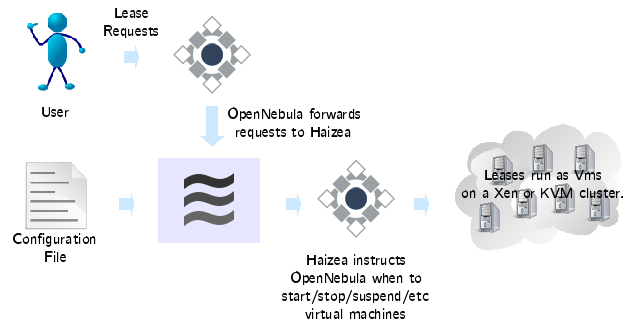
\includegraphics{images/mode_opennebula.png}
\end{center}

Haizea can be used as a drop-in replacement for OpenNebula's scheduling daemon. OpenNebula is a virtual infrastructure manager that enables the dynamic deployment and re-allocation of virtual machines on a pool of physical resources. OpenNebula and Haizea complement each other, since OpenNebula provides all the enactment muscle (OpenNebula can manage Xen and KVM virtual machines on a cluster, with VMWare support to follow shortly) while Haizea provides all the scheduling brains.

\subsection{Unattended simulation mode}

\begin{center}
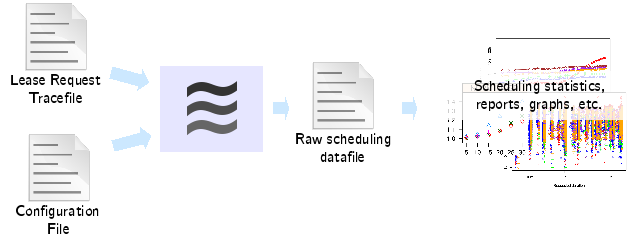
\includegraphics{images/mode_unattended_simulation.png}
\end{center}

In this mode, Haizea takes a list of lease requests (specified in a \emph{tracefile}) and a configuration file specifying simulation and scheduling options (such as the characteristics of the hardware to simulate), and processes them in ``simulated time''. In other words, the goal of this mode is to obtain the final schedule for a set of leases, without having to wait for all those leases to complete in real time (this makes this mode particularly useful to find out what effect a certain scheduling option could have over a period of weeks or months). In fact, the final result of an unattended simulation is a datafile with raw scheduling data and metrics which can be used to generate reports and graphs.

\subsection{Interactive simulation mode}

\begin{center}
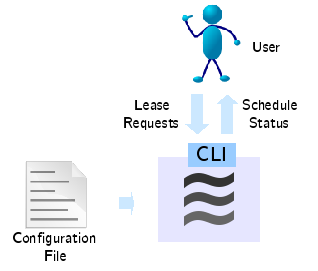
\includegraphics{images/mode_interactive_simulation.png}
\end{center}

In this mode, enactment actions are simulated, but Haizea runs in ``real time''. This means that, instead of having to provide a list of lease requests beforehand, your can use Haizea's command-line interface to request leases interactively and query the status of Haizea's schedule (e.g., to find out the state of lease you've requested). Obviously, this mode is not useful if you want to simulate weeks or months of requests, but it is handy if you want to experiment with leases and track the schedule in a more user-friendly way (since the datafile produced by the unattended simulation is mostly meant for consumption by other programs, e.g., to generate graphs and reports).

\section{Haizea architecture}

\begin{center}
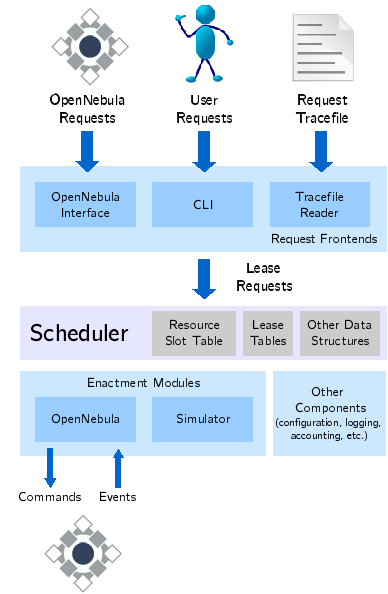
\includegraphics{images/architecture.png}
\end{center}

Haizea is divided into the following three layers:

\begin{description}
\item[The request frontend] This is where lease requests arrive. Haizea can currently accept requests from OpenNebula or read them from a tracefile (in SWF format or using the Haizea-specific LWF format). A command-line interface is in the works.
\item[The scheduling core] This is where the lease requests are processed and scheduled, resulting in enactment actions happening at specific points in time (e.g., "Start VM for lease X in node Y at time T", etc.)
\item[The enactment modules] These take care of the "dirty work" of carrying out the enactment actions generated by the scheduler. Haizea can currently send enactment actions to OpenNebula, resulting in Haizea being able to manage Xen and KVM clusters (VMWare support coming soon), or to a simulated cluster.
\end{description}
The Haizea architecture keeps these three layers completely decoupled, which means that adding support for an additional enactment backend only requires writing an enactment module for that backend. The API for enactment modules is still not fully defined, and integration with OpenNebula is currently driving this effort. However, if you'd be interested in using Haizea in another system, please do let us know. We'd be very interested in hearing what your requirements are for the frontend and enactment APIs.

\section{Haizea is still a technology preview}

Haizea started out as research software (and it is still largely meant for research purposes). Although Haizea works and we're getting to the point where it can be used in production systems, it is still a technology preview, so please use it with caution. In particular, although we've produced some documentation and polished up the code, there is still a fair amount of documentation that has to be produced. If you have any trouble using Haizea, or understanding any part of the source code, please don't hesitate to ask for help.